%%%%%%%%%%%%%%%%%%%%%%%%%%%%%%%%%%%%%%%%%%%%%%%%%%%%%%%%%%%%%%%%%%
%%  ~ Trabajo de Fin de Grado - Universidad de Vigo (ESEI) ~    %%
%% Autor: Diego Enrique Fontán Lorenzo                          %%
%% Tutor: Miguel Ramón Díaz-Cacho Medina                        %%
%% Convocatoria: Julio 2020/21                                  %%
%% Título: Framework de automatización de auditorías Red Team   %%
%%%%%%%%%%%%%%%%%%%%%%%%%%%%%%%%%%%%%%%%%%%%%%%%%%%%%%%%%%%%%%%%%%

%%%%%%%%%%%%%%%%%%%%%%%%%%%%%
%% The End (?)
%%%%%%%%%%%%%%%%%%%%%%%%%%%%%

\chapter{Epílogo} \label{cap:ending}

En este último capítulo se resumen las principales aportaciones de este proyecto según los objetivos descritos en el apartado \ref{sec:objetivos}, así como las conclusiones (tanto técnicas como personales) y las vías de trabajo futuro.\n

%%%%%%%%%%%%%%%%%%%%%%%%%%%%%
%% Main contributions
%%%%%%%%%%%%%%%%%%%%%%%%%%%%%

\section{Principales aportaciones} \label{sec:contributions}

Este trabajo aporta, principalmente, una nueva herramienta de código abierto. Dicha herramienta es capaz de automatizar las auditorías de seguridad, ofreciendo una gestión visual.\sn

Con esta acción se pretende, entre otras cosas, desmitificar el mundo del \textit{hacking}. Tanto los docentes, como aquellas personas que sientan interés por el tema, pueden obtener una manera sencilla de iniciarse en la materia. La aplicación es fácil de descargar y ejecutar, contando a su vez con una interfaz amigable e intuitiva.\sn

Por otro lado, se ha conseguido aportar una nueva aplicación con la que reemplazar muchas de las herramientas existentes en el mercado. Esto consigue reducir la cantidad de soluciones \textit{software} que necesita un \textit{pentester} para llevar a cabo auditorías de ciberseguridad.\sn

Por último, y aunque actualmente no sea una aportación real, se espera que se genere una nueva comunidad en torno al proyecto, la cual contribuya creando nuevos \textit{ingredientes} y \textit{recetas} que permitan realizar tareas cada vez más complejas.\n

%%%%%%%%%%%%%%%%%%%%%%%%%%%%%
%% Conclusions
%%%%%%%%%%%%%%%%%%%%%%%%%%%%%

\section{Conclusiones} \label{sec:conclusions}

En este punto, el autor del documento expondrá sus pensamientos en lo referente a la realización del proyecto, tanto desde una perspectiva técnica como desde un punto de vista personal.\n

\subsection{Conclusiones técnicas} \label{sec:techconclusions}

A pesar de no ser un práctica habitual por parte de los estudiantes, es increíble lo que el uso de metodologías (como pueden ser las descritas en el apartado \ref{sec:methodology}) son capaces de aportar a un proyecto. Como conclusiones técnicas, se destaca varios puntos:\sn

La aplicación de los conocimientos obtenidos durante la carrera, como pueden ser el análisis y el diseño de la aplicación, han conseguido minimizar la cantidad de errores que se producen normalmente durante la etapa de desarrollo.\sn

También es importante mencionar que gracias a las bases adquiridas, se ha conseguido hacer uso de herramientas y tecnologías que se ajustan a los requisitos y motivaciones del proyecto. Un ejemplo de esto son lenguajes de programación concurrentes con los que no se trabaja en la Universidad o la implementación de arquitecturas nunca antes vistas por el alumno.\sn

Algunos de los conocimientos adquiridos al realizar este trabajo, y que servirán de base para el futuro, son:\sn

- Aprender a implementar paradigmas de programación basadas en flujos de datos.\sn

- El descubrimiento de nuevos \textit{frameworks} que permitan un mejor diseño.\sn

- \LaTeX \textbf{ }como estándar para la maquetación de documentos académico-científicos.\sn

\subsection{Conclusiones personales} \label{sec:personalconclusions}

En un primer momento, la idea de desarrollar un programa similar a nuevo lenguaje de programación visual era bastante imponente. No sólo se aleja del tipo de proyectos que concebimos habitualmente, si no que la documentación relativa a la materia es bastante escasa y/o incompleta. Esto, unido al capricho de desarrollar la interfaz utilizando un \textit{framework} con el que nunca antes se había trabajado, suponía un reto ideal que encajaba perfectamente con la ideología de un Trabajo de Fin de Grado.\sn

Ahora, tras haber finalizado el proyecto y habiendo conseguido desarrollar una base sólida sobre la que hacer crecer la idea, el autor de este documento es consciente de que no existen ideas imposibles. El error suele estar solamente en un mal enfoque o una falta de motivación real para llevarlas a cabo.\sn

Por otro lado, es muy importante no olvidarse de que los grandes logros nunca se consiguen de manera individual. \emph{La informática no sólo se basa en relacionarse con ordenadores}. Al igual que en muchos otros aspectos de la vida, también es necesario que existan personas que te apoyen, aconsejen, critiquen y motiven para seguir adelante, pudiendo ofrecer cada vez mejores resultados\footnote{Gracias a mi tutor y a mi círculo de personas cercanas por hacérmelo tener siempre presente.}.

\newpage

%%%%%%%%%%%%%%%%%%%%%%%%%%%%%
%% Future
%%%%%%%%%%%%%%%%%%%%%%%%%%%%%

\section{Vías de trabajo futuro} \label{sec:future}

Durante el desarrollo del trabajo, se ha conseguido desarrollar las bases de la aplicación tal y como estaba previsto. Aún así, el \textit{software} presentado se trata de una versión inicial, sobre el cual se irán añadiendo nuevas mejoras. En este apartado se numeran algunas de ellas, a corto plazo.\sn

\subsection{Creación de nuevas \textit{recetas} e \textit{ingredientes}} \label{sub:newrecipesandingredients}

Actualmente la aplicación consta de los nodos básicos para demostrar la utilidad y eficacia de la misma. Es necesario que la aplicación siga creciendo y se mantenga actualizada. Para ello, una de las tareas a realizar es la creación de nuevos nodos, que extiendan su funcionalidad, así como crear un repositorio de plantillas en el cual poder compartir pruebas y metodologías usando la aplicación.\sn

Esta tarea irá desarrollándose de manera proporcional al interés que sienta la comunidad, tal y como se comenta en el último párrafo del apartado \ref{sec:contributions}.\sn

\subsection{\textit{Refactorización} del código}

Debido a que el proyecto fue desarrollado teniendo en cuenta una fecha límite, su implementación no es la más correcta. Es necesario revisar el código fuente para mejorar los mecanismos de seguridad y el rendimiento de sus componentes, entre otras cosas.\sn

\subsection{Creación de pruebas automatizadas}

En el apartado \ref{sub:varsprint1} se detalla el motivo por el cual el código no consta de prueba unitarias que aseguren su correcto funcionamiento. La creación de pruebas automatizadas es una de las partes fundamentales en el desarrollo de \textit{software} sostenible. Es por ello, que se pretende implementarlas en el futuro más próximo.\n

\begin{figure}[H]
    \centering
    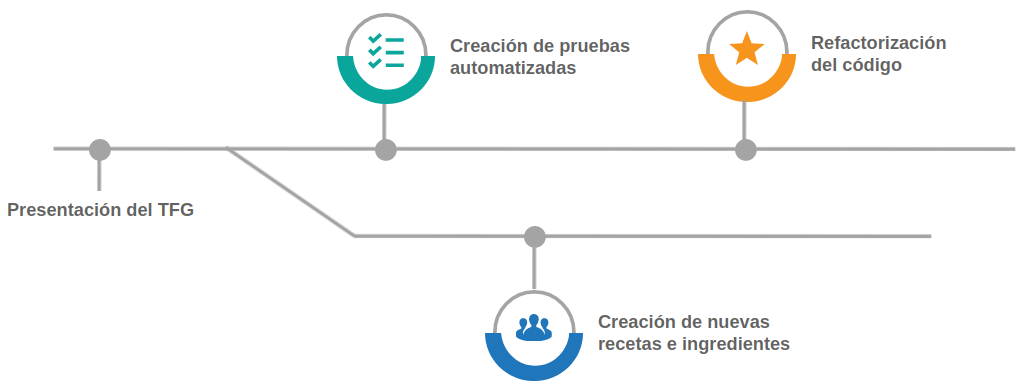
\includegraphics[width=13cm]{img/tables/37_Goals.png}
    \caption{Metas a corto plazo.}
    \label{fig:goals}
\end{figure}
